\documentclass{article}

\newif\ifanswers
\usepackage{fancyhdr}
\usepackage{lastpage}
\usepackage{extramarks}
\usepackage[usenames,dvipsnames]{color}
\usepackage{graphicx}
\usepackage{listings}
\usepackage{courier}
\usepackage{enumerate}
\usepackage{booktabs}
\usepackage{amsmath, amsthm, amssymb}
\usepackage{caption}
\usepackage{comment}
\usepackage{subcaption}
\captionsetup[table]{skip=4pt}
\usepackage{framed}
\usepackage{bm}
\usepackage{float}
\setcounter{section}{-1}



\usepackage{style}
\usepackage{xcolor}
\graphicspath{{img/}}
\usepackage{amsmath}
\usepackage{amsfonts}
\usepackage{amssymb}
\usepackage{hyperref}



\newenvironment{myitemize}
{ \begin{itemize}
		\setlength{\itemsep}{0pt}
		\setlength{\parskip}{0pt}
		\setlength{\parsep}{0pt}     }
	{ \end{itemize}                  }


\usepackage[backend=bibtex]{biblatex}
\addbibresource{papers.bib}

\usepackage{tikz}
\usetikzlibrary{positioning,patterns,fit}

\newcommand{\ifans}{\ifanswers \textbf{Solution: }}

\topmargin=-0.45in
\evensidemargin=0in
\oddsidemargin=0in
\textwidth=6.5in
\textheight=9.0in
\headsep=0.25in

\linespread{1.1}

\pagestyle{fancy}
\rhead{\hmwkAuthorName}
\lhead{\hmwkClass: \hmwkTitle}
\lfoot{\lastxmark}
\cfoot{}
\rfoot{Page\ \thepage\ of\ \protect\pageref{LastPage}}
\renewcommand\headrulewidth{0.4pt}
\renewcommand\footrulewidth{0.4pt}

\setlength\parindent{0pt}

\lstloadlanguages{Python}
\lstset{language=Python,
        frame=single,
        basicstyle=\footnotesize\ttfamily
        keywordstyle=[1]\color{Blue}\bf,
        keywordstyle=[2]\color{Purple},
        keywordstyle=[3]\color{Blue}\underbar,
        identifierstyle=,
        commentstyle=\usefont{T1}{pcr}{m}{sl}\color{MyDarkGreen}\small,
        stringstyle=\color{Purple},
        showstringspaces=false,
        tabsize=5,
        morekeywords={rand},
        morekeywords=[2]{on, off, interp},
        morekeywords=[3]{test},
        morecomment=[l][\color{Blue}]{...},
        numbers=left,
        firstnumber=1,
        numberstyle=\tiny\color{Blue}
        stepnumber=5
}

\newcommand{\perlscript}[2]{
\begin{itemize}
\item[]\lstinputlisting[caption=#2,label=#1]{#1.pl}
\end{itemize}
}

\newcommand{\hmwkTitle}{Assignment \#2}
\newcommand{\hmwkClass}{CS\ 234 Winter 2020}
\newcommand{\hmwkAuthorName}{}

\title{
\vspace{-1in}
\textmd{\textbf{\hmwkClass:\ \hmwkTitle}}}
\author{}
\date{} % Insert date here if you want it to appear below your name

\begin{document}

\maketitle
\vspace{-.5in}
\begin{framed}
{\bf Due date: February 5, 2020 at 11:59 PM (23:59) PST}
\\[1em]
These questions require thought, but do not require long answers. Please be as concise as possible.
\\[1em]
We encourage students to discuss in groups for assignments. We ask
that you abide by the university Honor Code and that of the Computer Science department. If you have discussed the problems with others,
please include a statement saying who you discussed problems with. Failure to follow these instructions
will be reported to the Office of Community Standards. We reserve the right to run a fraud-detection software on your code. Please refer to \href{http://web.stanford.edu/class/cs234/index.html}{website}, Academic Collaboration and Misconduct section for details about collaboration policy.

Please review any additional instructions posted on the assignment page. When you are ready to submit, please
follow the instructions on the course website. \textbf{Make sure you test your code using the
provided commands and do not edit outside of the marked areas.}
\\[1em]
You'll need to download the starter code and fill the appropriate functions following the instructions from the handout and the code's documentation. Training DeepMind's network on \texttt{Pong} takes roughly \textbf{12 hours on GPU}, so \textbf{please start early}! (Only a completed run will recieve full credit) We will give you access to an Azure GPU cluster. You'll find the setup instructions on the course assignment page.
\end{framed}
\section*{Introduction}

In this assignment we will implement deep Q-learning, following DeepMind's paper (\cite{mnih2015human} and \cite{mnih-atari-2013}) that learns to play Atari games from raw pixels. The purpose is to demonstrate the effectiveness of deep neural networks as well as some of the techniques used in practice to stabilize training and achieve better performance. In the process, you'll become familiar with TensorFlow. We will train our networks on the \texttt{Pong-v0} environment from OpenAI gym, but the code can easily be applied to any other environment. \\

In Pong, one player scores if the ball passes by the other player. An episode is over when one of the players reaches $21$ points. Thus, the total return of an episode is between $-21$ (lost every point) and $+21$ (won every point). Our agent plays against a decent hard-coded AI player. Average human performance is $-3$ (reported in \cite{mnih-atari-2013}). In this assignment, you will train an AI agent with super-human performance, reaching at least $+10$ (hopefully more!).

\newpage
\section{Test Environment (6 pts)}
Before running our code on Pong, it is crucial to test our code on a test environment. In this problem, you will reason about optimality in the provided test environment by hand; later, to sanity-check your code, you will verify that your implementation is able to achieve this optimality. You should be able to run your models on CPU in no more than a few minutes on the following environment:

\begin{itemize}
\item $ 4 $ states: $ 0, 1, 2, 3 $
\item $ 5 $ actions: $ 0, 1, 2, 3, 4 $. Action $ 0 \leq i \leq 3 $ goes to state $ i $, while action $ 4 $ makes the agent stay in the same state.
\item Rewards: Going to state $ i $ from states 0, 1, and 3 gives a reward $R(i) $, where $R(0) = 0.1, R(1) = -0.2, R(2) = 0, R(3) = -0.1 $. If we start in state $ 2 $, then the rewards defind above are multiplied by $ - 10 $.  See Table~\ref{tab:TestEnv} for the full transition and reward structure.
\item One episode lasts 5 time steps (for a total of 5 actions) and always starts in state $ 0 $ (no rewards at the initial state).
\end{itemize}

\begin{center}
    \begin{tabular}{ | l | l | l | l |}
    \hline
    State ($s$) & Action ($a$) & Next State ($s'$) & Reward ($R$) \\ \hline
    0 & 0 & 0 & 0.1    \\ \hline
    0 & 1 & 1 & -0.2   \\ \hline
    0 & 2 & 2 & 0.0 \\ \hline
    0 & 3 & 3 & -0.1 \\ \hline
    0 & 4 & 0 & 0.1 \\ \hline
    1 & 0 & 0 & 0.1    \\ \hline
    1 & 1 & 1 & -0.2   \\ \hline
    1 & 2 & 2 & 0.0 \\ \hline
    1 & 3 & 3 & -0.1 \\ \hline
    1 & 4 & 1 & -0.2 \\ \hline
    2 & 0 & 0 & -1.0    \\ \hline
    2 & 1 & 1 & 2.0   \\ \hline
    2 & 2 & 2 & 0.0 \\ \hline
    2 & 3 & 3 & 1.0 \\ \hline
    2 & 4 & 2 & 0.0 \\ \hline
    3 & 0 & 0 & 0.1    \\ \hline
    3 & 1 & 1 & -0.2   \\ \hline
    3 & 2 & 2 & 0.0 \\ \hline
    3 & 3 & 3 & -0.1 \\ \hline
    3 & 4 & 3 & -0.1 \\ \hline
    \end{tabular}
\captionof{table}{Transition table for the Test Environment} \label{tab:TestEnv}
\end{center}

An example of a trajectory (or episode) in the test environment is shown in Figure \ref{fig:test_env}, and the trajectory can be represented in terms of $s_t, a_t, R_t$ as:
$s_0 = 0, a_0=1, R_0 = -0.2, s_1=1, a_1=2, R_1 = 0, s_2=2, a_2=4, R_2 = 0, s_3=2, a_3=3, R_3 = (-0.1)\cdot(-10) = 1, s_4=3, a_4=0, R_4 = 0.1, s_5=0 $.

\begin{figure}[H]
  \centering
  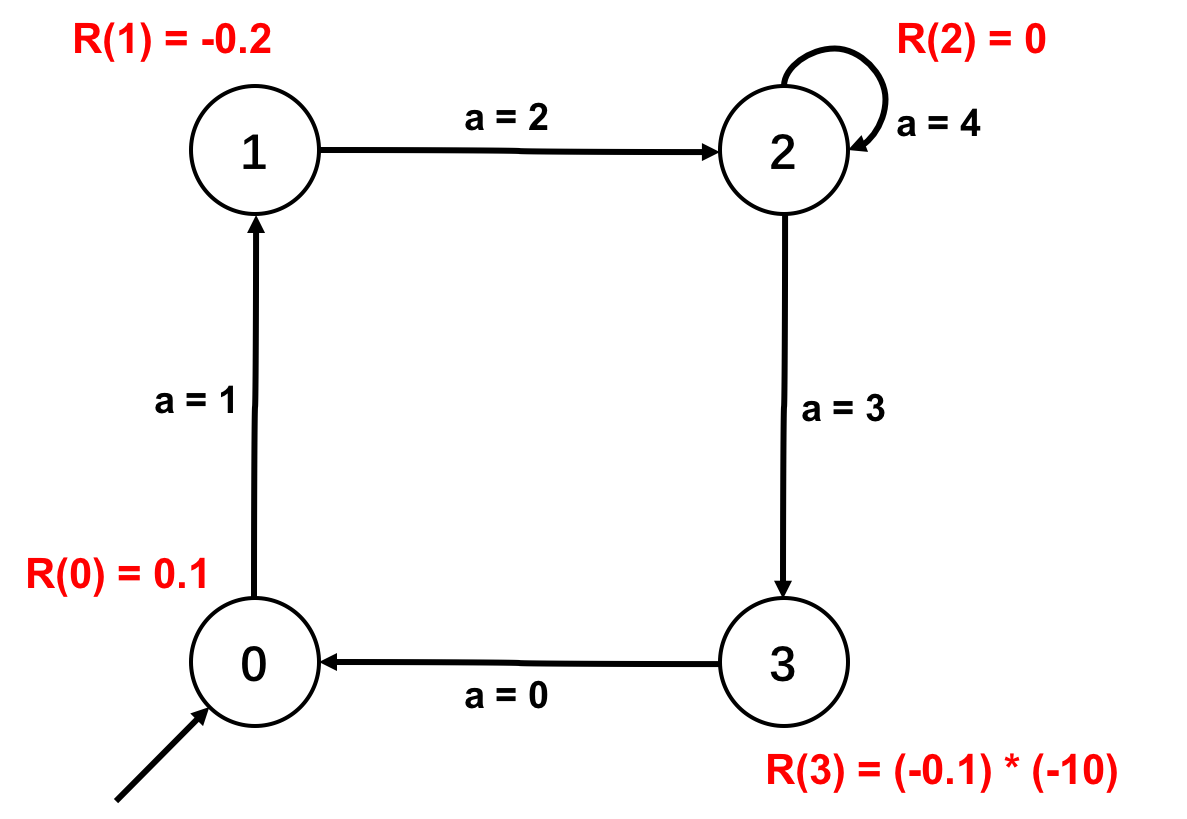
\includegraphics[width=.45\linewidth]{test_env}
  \caption{Example of a trajectory in the Test Environment}
  \label{fig:test_env}
\end{figure}

\begin{enumerate}
\item (\textbf{written} 6 pts) What is the maximum sum of rewards that can be achieved in a single trajectory in the test environment, assuming $\gamma = 1$? Show first that this value is attainable in a single trajectory, and then briefly argue why no other trajectory can achieve greater cumulative reward.
\end{enumerate}

\textbf{Answer:}

The maximum cumulative reward valut is: 4.1

$ {(0, 2, 0.0), (2, 1, 2.0), (1, 2, 0.0), (2, 1, 2.0), (1, 0, 0.1)} $

The maximun single step reward value we can get is (2, 1, 2.0), within 5 steps starting from state 0, we can only do this 2 times at maximum, and by doing this, we can get 4.0 reward.

For the 1 or 2 steps left, we can only do (0, 2, ... , other) or (0, other, 2, ...) they could maximumly have same reward value 0.1

\section{Q-Learning (24 pts)}\label{q-learn}

\paragraph{Tabular setting}
If the state and action spaces are sufficiently small, we can simply maintain a table containing the value of $Q(s,a)$ -- an estimate of $Q^*(s,a)$ -- for every $(s,a)$ pair.
In this \emph{tabular setting}, given an experience sample $ (s, a, r, s') $, the update rule is
\begin{equation}
\label{eq1}
\begin{split}
Q(s,a) &\leftarrow Q(s,a) + \alpha\left(r+\gamma \max_{a' \in \mathcal{A}}Q\left(s',a' \right) - Q\left(s, a\right)\right)
\end{split}
\end{equation}
where $\alpha > 0$ is the learning rate, $\gamma \in [0,1)$ the discount factor.

\paragraph{Approximation setting}
Due to the scale of Atari environments, we cannot reasonably learn and store a Q value for each state-action tuple. We will instead represent our Q values as a function $ \hat{q}(s, a; \mathbf{w}) $ where $ \mathbf{w} $ are parameters of the function (typically a neural network's weights and bias parameters). In this \emph{approximation setting}, the update rule becomes
\begin{equation}
\label{eq2}
\mathbf{w} \leftarrow \mathbf{w} + \alpha\left(r+\gamma \max_{a' \in \mathcal{A}} \hat{q}\left(s', a'; \mathbf{w} \right) - \hat{q}\left(s, a; \mathbf{w} \right)\right) \nabla_{\mathbf{w}}\hat{q}(s, a; \mathbf{w}).
\end{equation}
In other words, we aim to minimize
\begin{equation}
L(\mathbf{w}) = \underset{s,a,r,s' \sim \mathcal{D}}{\mathbb{E}}\left[\left(r+\gamma \max_{a' \in \mathcal{A}}\hat{q}\left(s', a'; \mathbf{w} \right) - \hat{q}(s, a; \mathbf{w})\right)^2\right]
\end{equation}

\paragraph{Target Network}
DeepMind's paper \cite{mnih2015human} \cite{mnih-atari-2013} maintains two sets of parameters, $\mathbf{w}$ (to compute $ \hat{q}(s, a)$) and $\mathbf{w}^-$ (target network, to compute $ \hat{q}(s', a') $) such that our update rule becomes
 \begin{equation}
\mathbf{w} \leftarrow \mathbf{w} + \alpha\left(r+\gamma \max_{a' \in \mathcal{A}}\hat{q}\left(s', a'; \mathbf{w}^- \right) - \hat{q}\left(s, a; \mathbf{w} \right)\right) \nabla_{\mathbf{w}} \hat{q}(s, a; \mathbf{w}).
\end{equation}
and the corresponding optimization objective becomes
\begin{equation}
L^{-}(\mathbf{w}) = \underset{s,a,r,s' \sim \mathcal{D}}{\mathbb{E}}\left[\left(r+\gamma \max_{a' \in \mathcal{A}}\hat{q}\left(s', a'; \mathbf{w^-} \right) - \hat{q}(s, a; \mathbf{w})\right)^2\right]
\end{equation}

The target network's parameters are updated to match the Q-network's parameters every $C$ training iterations, and are kept fixed between individual training updates.

\paragraph{Replay Memory}
As we play, we store our transitions $ (s, a, r, s') $ in a buffer $\mathcal{D}$. Old examples are deleted as we store new transitions. To update our parameters, we \emph{sample} a minibatch from the buffer and perform a stochastic gradient descent update.

\paragraph{$\epsilon$-Greedy Exploration Strategy}
For exploration, we use an $\epsilon$-greedy strategy.
This means that with probability $\epsilon$, an action is chosen uniformly at random from $\mathcal{A}$, and with probability $1-\epsilon$, the greedy action (i.e., $\arg\max_{a \in \mathcal{A}} \hat{q}(s,a,\mathbf{w})$) is chosen. DeepMind's paper \cite{mnih2015human} \cite{mnih-atari-2013} linearly anneals $ \epsilon $ from $1$ to $0.1$ during the first million steps. At test time, the agent chooses a random action with probability $\epsilon_{\text{soft}} = 0.05$.\\

There are several things to be noted:
\begin{itemize}
\item In this assignment, we will update $\mathbf{w}$ every \texttt{learning\_freq} steps by using a \texttt{minibatch} of experiences sampled from the replay buffer.

\item DeepMind's deep Q network takes as input the state $s$ and outputs a vector of size $|\mathcal{A}|$. In the \texttt{Pong} environment, we have $|\mathcal{A}| = 6$ actions, so $\hat{q}(s; \mathbf{w}) \in \mathbb{R}^{6}$.

\item The input of the deep Q network is the concatenation $4$ consecutive steps, which results in an input after preprocessing of shape $(80 \times 80 \times 4)$.
\end{itemize}

We will now examine these assumptions and implement the $\epsilon$-greedy strategy.

\begin{enumerate}

\item (\textbf{written} 3 pts) What is one benefit of representing the $Q$ function as $\hat{q}(s; \mathbf{w}) \in \mathbb{R}^{|\mathcal{A}|}$?

\textbf{Answer:}

This representation integrate $a \in |\mathcal{A}|$ into parameter $\mathbf{w}$.

By doing this for each state we don't need to to try all the actions and get $\max_{a' \in \mathcal{A}}\hat{q}\left(s', a'; \mathbf{w} \right)$

Instead for each state, we only need a single interaction.


\item (\textbf{coding} 3 pts) Implement the \texttt{get\_action} and \texttt{update} functions in \texttt{q1\_schedule.py}. Test your implementation by running \texttt{python q1\_schedule.py}.
\end{enumerate}

We will now investigate some of the theoretical considerations involved in the tuning of the hyperparameter $C$ which determines the frequency with which the target network weights $\mathbf{w^-}$ are updated to match the Q-network weights $\mathbf{w}$. On one extreme, the target network could be updated \textit{every} time the Q-network is updated; it's straightforward to check that this reduces to not using a target network at all. On the other extreme, the target network could remain fixed throughout the entirety of training.\\

Furthermore, recall that stochastic gradient descent minimizes an objective of the form $J(\mathbf{w}) = \mathbb{E}_{x \sim \mathcal{D}}[l(x,\mathbf{w})]$ by making sample updates of the following form:
\[
\mathbf{w} \leftarrow \mathbf{w} - \alpha \nabla_{\mathbf{w}}l(x,\mathbf{w})
\]
Stochastic gradient descent has many desirable theoretical properties; in particular, under mild assumptions, it is known to converge to a local optimum. In the following questions we will explore the conditions under which Q-Learning constitutes a stochastic gradient descent update.

\begin{enumerate}
\setcounter{enumi}{2}
\item (\textbf{written} 5 pts) Consider the first of these two extremes: standard Q-Learning without a target network, whose weight update is given by equation \textbf{(2)} above. Is this weight update an instance of stochastic gradient descent (up to a constant factor of 2) on the objective $L(\mathbf{w})$ given by equation \textbf{(3)}? Argue mathematically why or why not.

\item (\textbf{written} 5 pts) Now consider the second of these two extremes: using a target network that is never updated (i.e. held fixed throughout training). In this case, the weight update is given by equation \textbf{(4)} above, treating $\mathbf{w^-}$ as a constant. Is this weight update an instance of stochastic gradient descent (up to a constant factor of 2) on the objective $L^{-}(\mathbf{w})$ given by equation \textbf{(5)}? Argue mathematically why or why not.

\item (\textbf{written} 3 pts) An obvious downside to holding the target network fixed throughout training is that it depends on us knowing good weights for the target network \textit{a priori}; but if this was the case, we wouldn't need to be training a Q-network at all! In light of this, together with the discussion above regarding the convergence of stochastic gradient descent and your answers to the previous two parts, describe the fundamental tradeoff at play in determining a good choice of $C$.

\item (\textbf{written}, 5 pts) In supervised learning, the goal is typically to minimize a predictive model's error on data sampled from some distribution.
If we are solving a regression problem with a one-dimensional output, and we use mean-squared error to evaluate performance, the objective writes
\[
L(\mathbf{w}) = \underset{(\mathbf{x},y) \sim \mathcal{D}}{\mathbb{E}}[(y - f(\mathbf{x}; \mathbf{w}))^2]
\]
where $\mathbf{x}$ is the input, $y$ is the output to be predicted from $\mathbf{x}$, $\mathcal{D}$ is a dataset of samples from the (unknown) joint distribution of $\mathbf{x}$ and $y$, and $f(\cdot; \mathbf{w})$ is a predictive model parameterized by $\mathbf{w}$.

This objective looks very similar to the DQN objective stated above.
How are these two scenarios different? Hint: how does this dataset $\mathcal{D}$ differ from the replay buffer $\mathcal{D}$ used above?
\end{enumerate}


\section{Linear Approximation (24 pts)}
\begin{enumerate}
\item (\textbf{written}, 3 pts) Show that Equations (1) and (2) from problem 1 above are exactly the same when  $\hat{q}(s, a; \mathbf{w}) = \mathbf{w}^\top \delta(s,a)$, where $\mathbf{w} \in \mathbb{R}^{\vert\mathcal{S}\vert \vert \mathcal{A}\vert }$ and $\delta : \mathcal{S} \times \mathcal{A} \rightarrow \mathbb{R}^{|\mathcal{S}| |\mathcal{A}|}$ with
\[
    [\delta(s,a)]_{s',a'}=\left\{
                \begin{array}{ll}
                  1 & \text{ if } s'=s, a'=a\\
                  0 & \text{otherwise}\\
                \end{array}
              \right.
  \]

\item (\textbf{written}, 3 pts) Assuming $\hat{q}(s, a; \mathbf{w})$ takes the form specified in the previous part, compute $\nabla_{\mathbf{w}} \hat{q}(s, a; \mathbf{w})$ and write the update rule for $\mathbf{w}$.


 \item (\textbf{coding}, 15 pts) We will now implement linear approximation in TensorFlow. This question will set up the pipeline for the remainder of the assignment. You'll need to implement the following functions in \texttt{q2\_linear.py} (please read through \texttt{q2\_linear.py}):
\begin{itemize}
	\item \texttt{add\_placeholders\_op}
	\item \texttt{get\_q\_values\_op}
	\item \texttt{add\_update\_target\_op}
	\item \texttt{add\_loss\_op}
	\item \texttt{add\_optimizer\_op}
\end{itemize}
Test your code by running \texttt{python q2\_linear.py} \textbf{locally on CPU}.  This will run linear approximation with TensorFlow on the test environment from Problem 0.  Running this implementation should only take a minute or two.

 \item (\textbf{written}, 3 pts) Do you reach the optimal achievable reward on the test environment? Attach the plot \texttt{scores.png} from the directory \texttt{results/q2\_linear} to your writeup.

\end{enumerate}


\section{Implementing DeepMind's DQN (13 pts)}

\begin{enumerate}

\item (\textbf{coding}, 10 pts) Implement the deep Q-network as described in \cite{mnih2015human} by implementing \texttt{get\_q\_} \texttt{values\_op} in \texttt{q3\_nature.py}. The rest of the code inherits from what you wrote for linear approximation. Test your implementation \textbf{locally on CPU} on the test environment by running \texttt{python q3\_nature.py}.  Running this implementation should only take a minute or two.

\item (\textbf{written}, 3 pts) Attach the plot of scores, \texttt{scores.png}, from the directory \texttt{results/q3\_nature} to your writeup. Compare this model with linear approximation. How do the final performances compare? How about the training time?
\end{enumerate}

\section{DQN on Atari (21 pts)}

Reminder: Please remember to kill your VM instances when you are done using them!! \\

The Atari environment from OpenAI gym returns observations (or original frames) of size $ (210 \times 160 \times 3) $, the last dimension corresponds to the RGB channels filled with values between $ 0 $ and $ 255 $ (\texttt{uint8}). Following DeepMind's paper \cite{mnih2015human}, we will apply some preprocessing to the observations:
\begin{myitemize}
\item Single frame encoding: To encode a single frame, we take the maximum value for each pixel color value over the frame being encoded and the previous frame. In other words, we return a pixel-wise max-pooling of the last 2 observations.
\item Dimensionality reduction: Convert the encoded frame to grey scale, and rescale it to $(80 \times 80 \times 1)$. (See Figure \ref{fig:pong_env})
\end{myitemize}

The above preprocessing is applied to the 4 most recent observations and these encoded frames are stacked together to produce the input (of shape $(80 \times 80 \times 4)$) to the Q-function. Also, for each time we decide on an action, we perform that action for 4 time steps. This reduces the frequency of decisions without impacting the performance too much and enables us to play 4 times as many games while training. You can refer to the \textit{Methods} section of \cite{mnih2015human} for more details.       \\

\begin{figure}[H]
\centering
\begin{subfigure}[b]{.5\textwidth}
  \centering
  
\includegraphics[width=.25\linewidth]{pong}
  \caption{Original input $ (210 \times 160 \times 3) $ with RGB colors}
  \label{fig:pong}
\end{subfigure}
\begin{subfigure}[b]{.5\textwidth}
  \centering
  
\includegraphics[width=.15\linewidth]{pong_grey}
  \caption{After preprocessing in grey scale of shape $ (80 \times 80 \times 1 ) $}
  \label{fig:pong_grey}
\end{subfigure}
\caption{\texttt{Pong-v0} environment}
\label{fig:pong_env}
\end{figure}

\begin{enumerate}

\item (\textbf{coding and written}, 5 pts). Now we're ready to train on the Atari \texttt{Pong-v0} environment. First, launch linear approximation on pong with \texttt{python q4\_train\_atari\_linear.py} \textbf{on Azure's GPU}. This will train the model for 500,000 steps and should take approximately an hour.  Briefly qualitatively describe how your agent's performance changes over the course of training. Do you think that training for a larger number of steps would likely yield further improvements in performance? Explain your answer.

\item (\textbf{coding and written}, 10 pts). In this question, we'll train the agent with DeepMind's architecture on the Atari \texttt{Pong-v0} environment. Run \texttt{python q5\_train\_atari\_nature.py} \textbf{on Azure's GPU}.  This will train the model for 5 million steps and should take around \textbf{12 hours}.  Attach the plot \texttt{scores.png} from the directory \texttt{results/q5\_train\_atari\_nature} to your writeup.
You should get a score of around 13-15 after 5 million time steps.  As stated previously, the DeepMind paper claims average human performance is $ -3 $.


As the training time is roughly 12 hours, you may want to check after a few epochs that your network is making progress.  The following are some training tips:

\begin{myitemize}
\item If you terminate your terminal session, the training will stop.  In order to avoid this, you should use \texttt{screen} to run your training in the background.
\item The evaluation score printed on terminal should start at -21 and increase.
\item The max of the q values should also be increasing.
\item The standard deviation of q shouldn't be too small. Otherwise it means that all states have similar q values.
\item You may want to use Tensorboard to track the history of the printed metrics. You can monitor your training with Tensorboard by typing the command \texttt{tensorboard --logdir=results} and then connecting to \texttt{ip-of-you-machine:6006}.  Below are our Tensorboard graphs from one training session:
\end{myitemize}

\begin{figure}[H]
\centering
	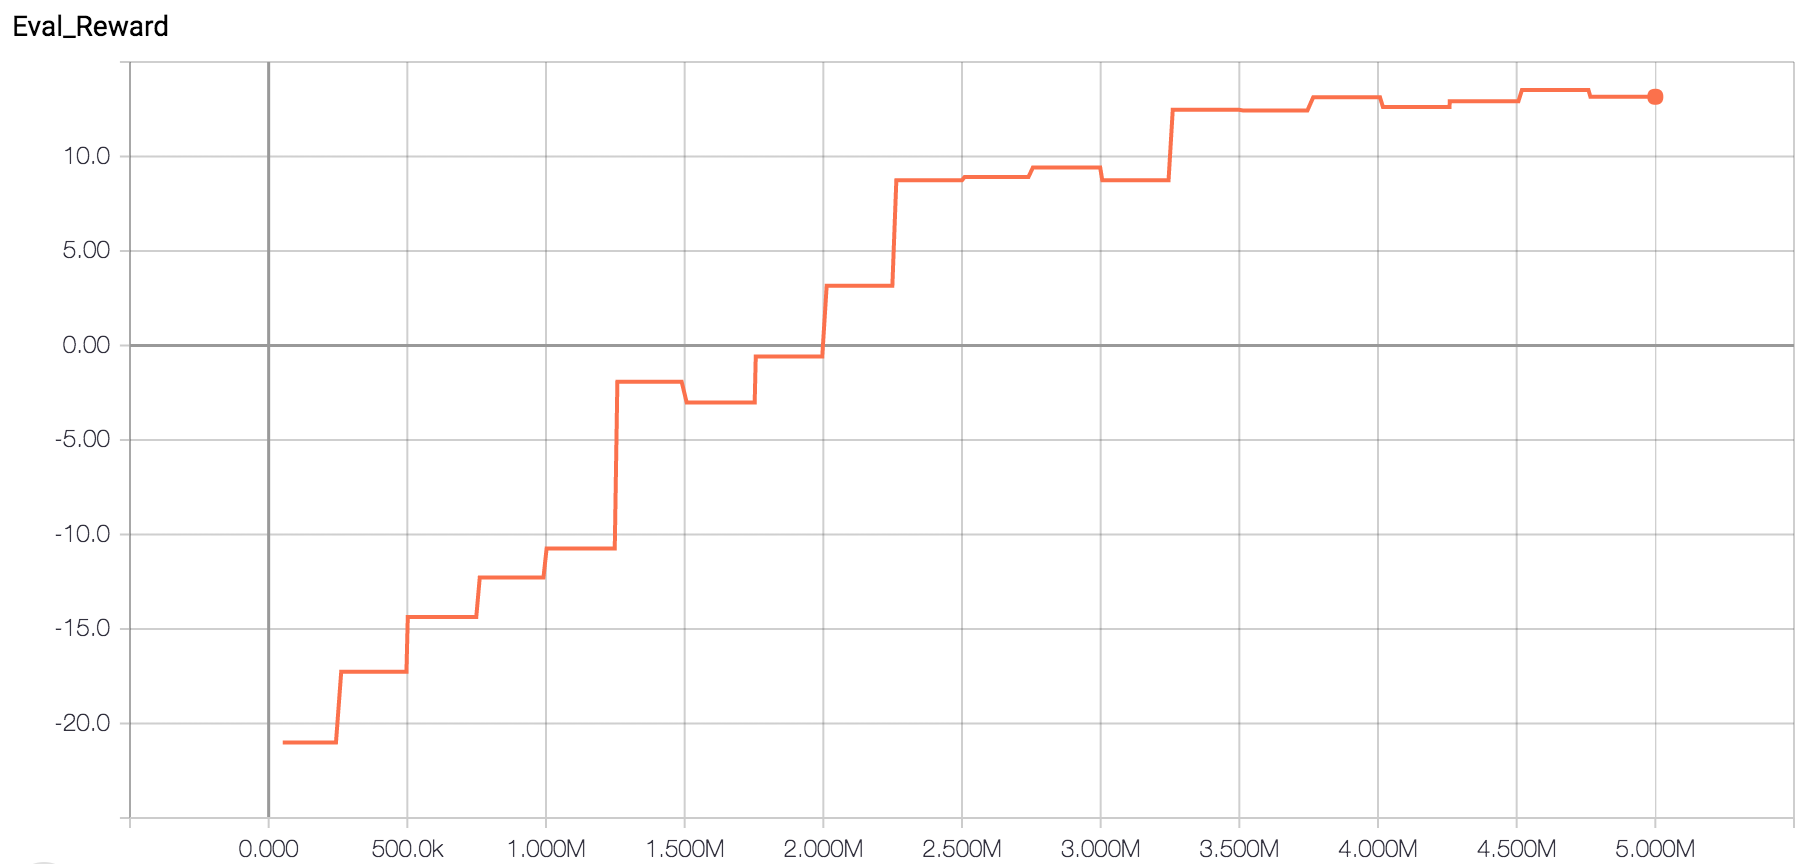
\includegraphics[width=.4\linewidth]{Eval_R.png}
	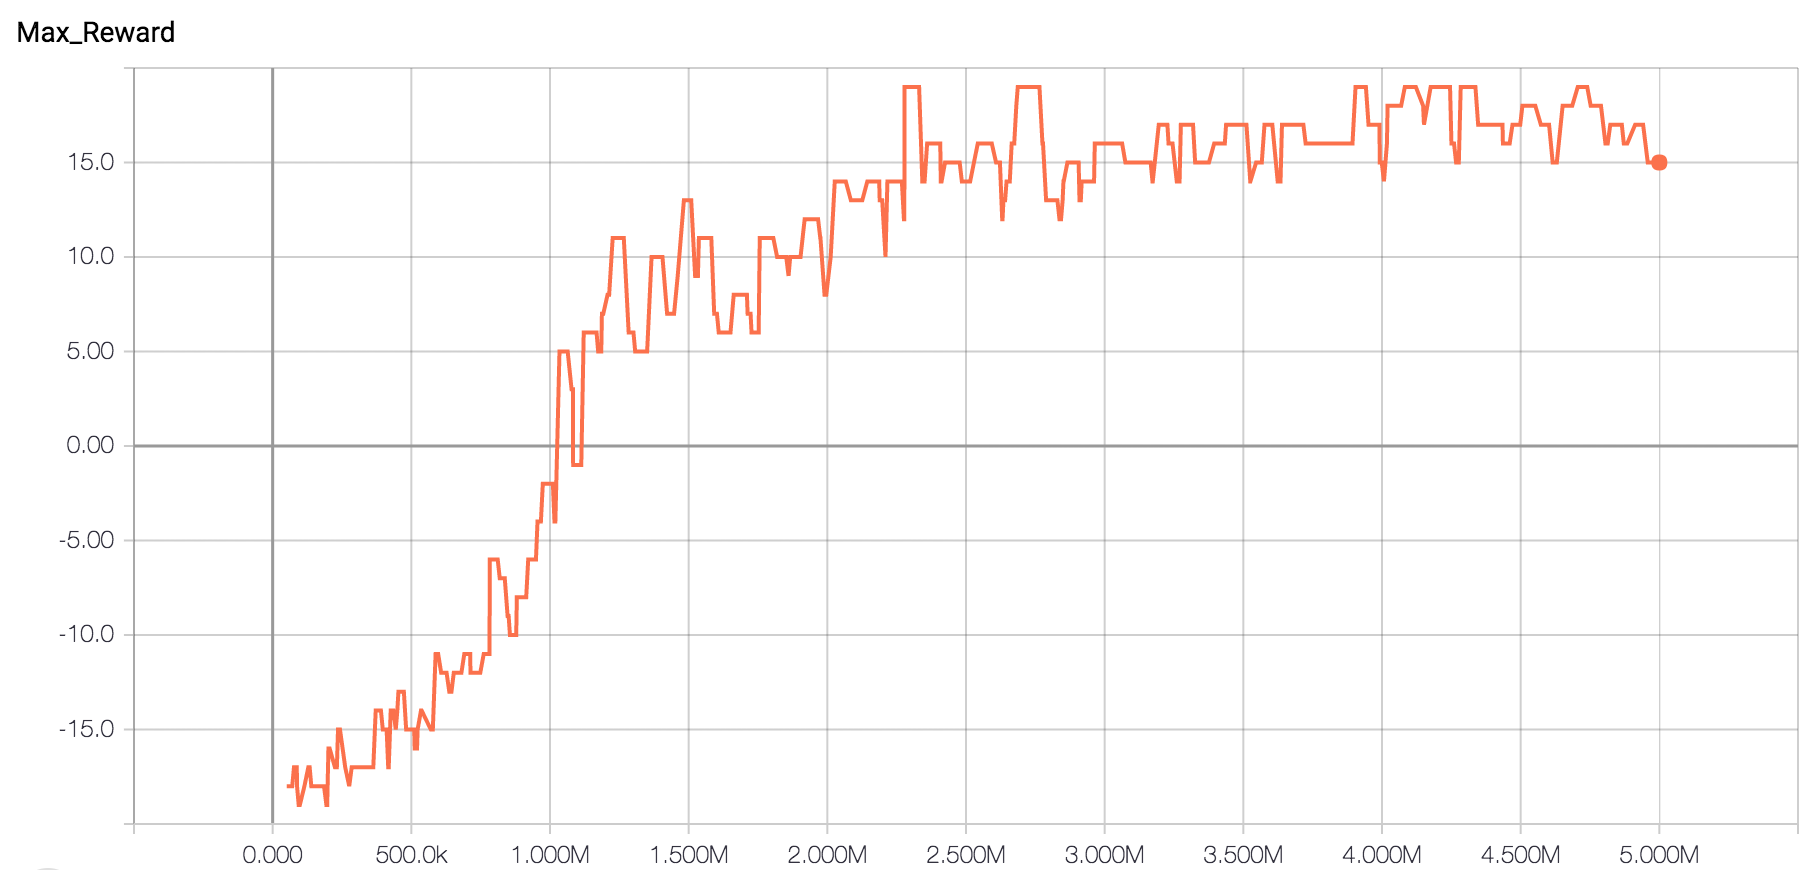
\includegraphics[width=.4\linewidth]{Max_R.png}
	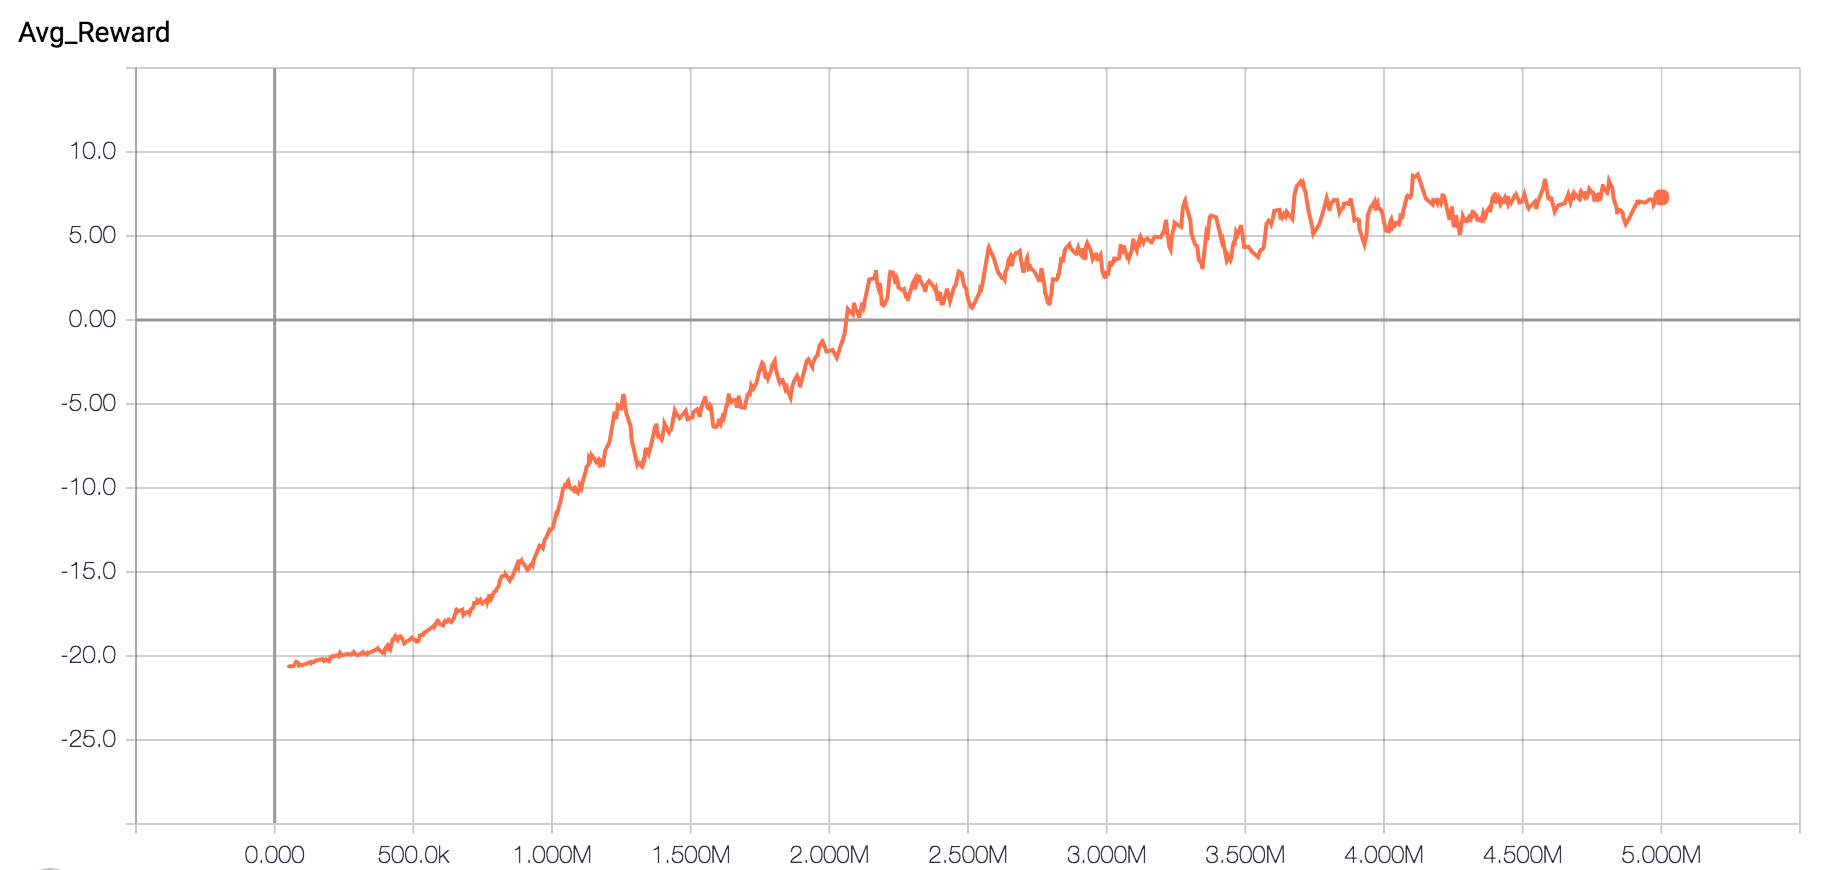
\includegraphics[width=.4\linewidth]{Avg_R.png}
	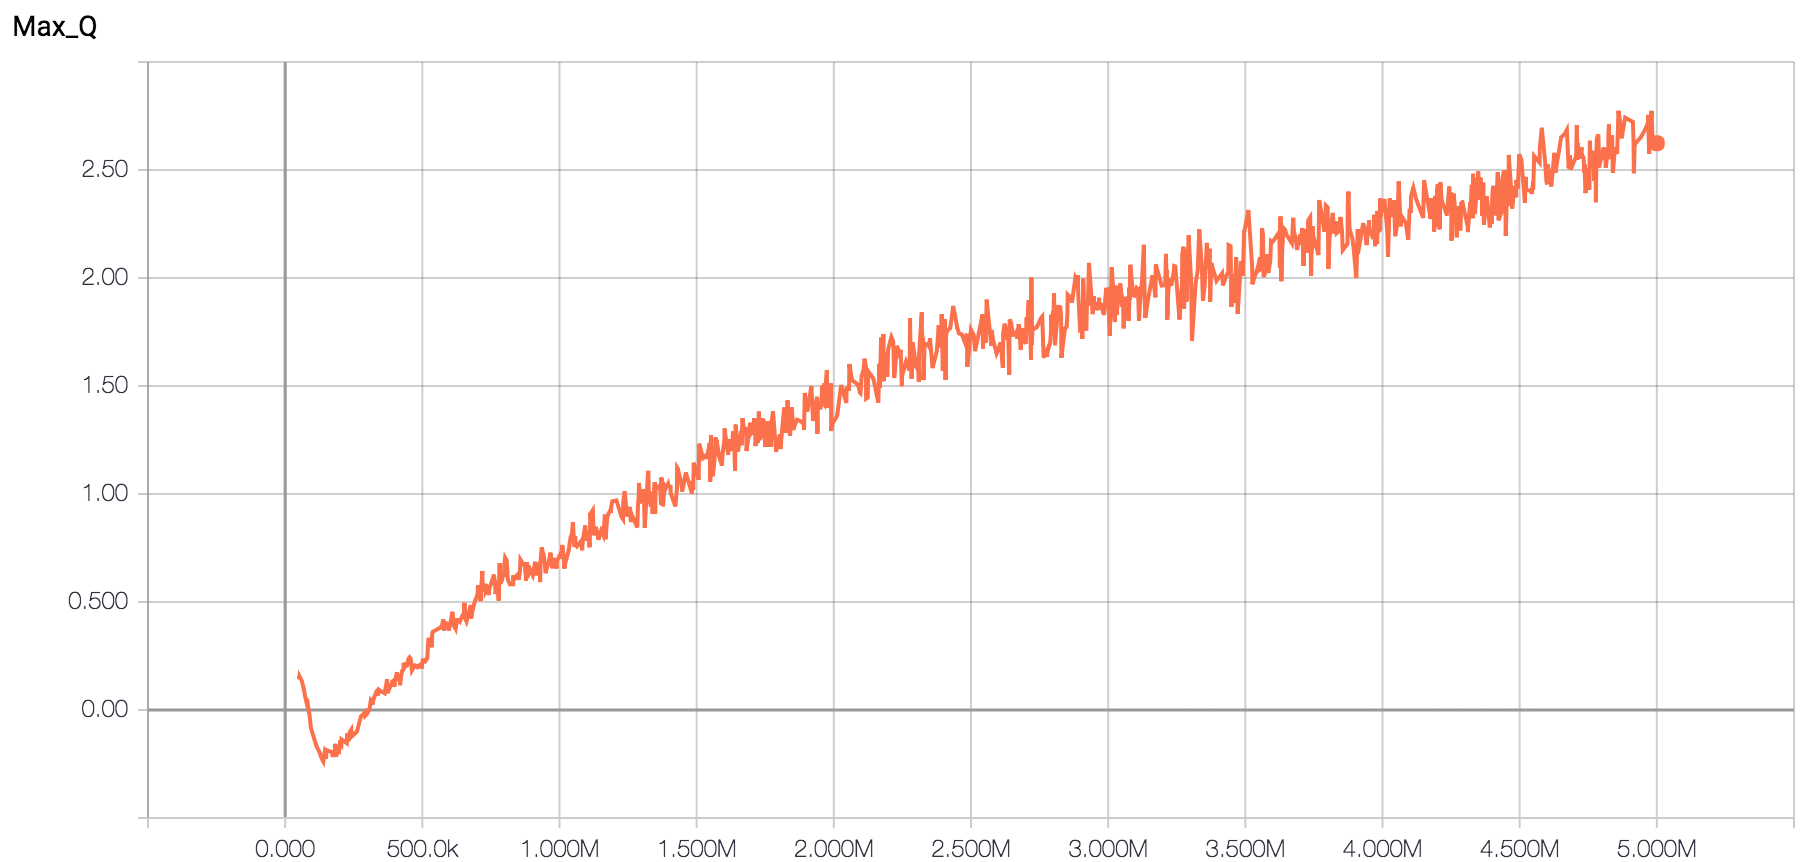
\includegraphics[width=.4\linewidth]{Max_Q.png}
\end{figure}

\item (\textbf{written}, 3 pts) In a few sentences, compare the performance of the DeepMind DQN architecture with the linear Q value approximator. How can you explain the gap in performance?

\item (\textbf{written}, 3 pts) Will the performance of DQN over time always improve monotonically? Why or why not?
\end{enumerate}

\section{$n$-step Estimators (12 pts)}
We can further understand the effects of using a bootstrapping target by adopting a statistical perspective. As seen in class, the Monte Carlo (MC) target is an unbiased estimator\footnote{Recall that the bias of an estimator is equal to the difference between the expected value of the estimator and the quantity which it is estimating. An estimator is unbiased if its bias is zero.} of the true state-action value, but it suffers from high variance. On the other hand, temporal difference (TD) targets are biased due to their dependence on the current value estimate, but they have relatively lower variance.

There exists a spectrum of target quantities which bridge MC and TD. Consider a trajectory $s_1,a_1,r_1,s_2,a_2,r_2,\ldots$ obtained by behaving according to some policy $\pi$. Given a current estimate $\hat{q}$ of $Q^{\pi}$, let the \textbf{$n$-step SARSA target} (in analogy to the TD target) be defined as:
\[
r_t + \gamma r_{t+1} + \gamma^2 r_{t+2} + \ldots + \gamma^{n-1}r_{t + n -1} + \gamma^{n}\hat{q}(s_{t+n},a_{t+n})
\]

(Recall that the 1-step SARSA target is given by $r_t + \gamma \hat{q}(s_{t+1},a_{t+1})$).\\

Given that the $n$-step SARSA target depends on fewer sample rewards than the MC estimator, it is reasonable to expect it to have lower variance. However, the improved bias of this target over the standard (i.e. 1-step) SARSA target may be less obvious.

\begin{enumerate}
\item (\textbf{written}, 12 pts) Prove that for a given policy $\pi$ in an infinite-horizon MDP, the $n$-step SARSA target is a less-biased (in absolute value) estimator of the true state-action value function $Q^{\pi}(s_t,a_t)$ than is the 1-step SARSA target. Assume that $n \geq 2$ and $\gamma < 1$. Further, assume that the current value estimate $\hat{q}$ is uniformly biased across the state-action space (that is, Bias($\hat{q}(s, a$)) $=$ Bias($\hat{q}(s', a'$)) for all states $s, s' \in \mathcal{S}$ and all actions $a, a' \in\mathcal{A}$). You need not assume anything about the specific functional form of $\hat{q}$.
\end{enumerate}

\printbibliography

\end{document}
